\documentclass[11pt]{article}
\usepackage[margin=1in]{geometry}
\usepackage[T1]{fontenc}
\usepackage{lmodern,microtype,amsmath,amssymb,booktabs,graphicx}
\usepackage{xcolor,hyperref,url}
\usepackage{placeins}
\renewcommand{\topfraction}{0.95}
\renewcommand{\bottomfraction}{0.95}
\renewcommand{\textfraction}{0.05}
\renewcommand{\floatpagefraction}{0.8}
\hypersetup{colorlinks=true,linkcolor=blue,urlcolor=blue}
\providecommand{\reportbuilddatetime}{unknown}
\InputIfFileExists{build-info.tex}{}{}
\newcommand{\resultgenerated}{2026-10-20 14:58:50 EDT}
\newcommand{\resultkey}{\texttt{e908a76f79f11ced}}

\newcommand{\dimensiongenerated}{2026-10-20 16:31:21 EDT}
\newcommand{\dimensionfittedpairs}{290,266}
\newcommand{\dimensionomittedpairs}{833,984}
\newcommand{\dimensionfittedfraction}{25.82}

\title{Relative-distance error and regional sparse SGD\\
in retinal embeddings}
\author{\small\begin{minipage}{0.94\textwidth}\centering
Source: \path{~/current_projects/grip/vignettes/articles/retinal-relative-stress/main.tex}
\end{minipage}}
\date{Build: \reportbuilddatetime}
\begin{document}
\maketitle

\section{The question}
An embedding of 120,804 retinal cells, fitted by stochastic gradient descent
(SGD) using 2,000 landmarks, did not show a steady decrease in independently
evaluated relative-distance error during its first 110 epochs. Does this
indicate an optimization failure, or are the fitting procedure and evaluation
measuring different things?

There are two separate issues. Sequential pair corrections need not decrease a
whole-data error after every pass. More importantly, the regional sparse method
uses selected pairs and unequal endpoint weights. It is therefore not the same
calculation as minimizing the equally weighted, all-pairs relative stress.
The scalar sparse diagnostic reported by the implementation is a useful
summary, but is not generally a potential function for its asymmetric updates.

This article derives that distinction and tests it on a deliberately small
retinal subset. Three methods are compared: regional sparse SGD with 25
landmarks, regional sparse SGD with 200 landmarks, and all-pairs SGD with
inverse-squared distance weights. All methods use the same three starting
configurations, original-space targets, and evaluation pairs.
An additional experiment varies output dimension from 3 to 300 on the same
cells, now using distances in 1,814 PCs. It asks how much error falls when
more output coordinates are available, and why the fitting proxy can still
give a different ranking from the all-pairs score.
The full 120,804-cell run remains paused at epoch 110; the experiment below
neither continues nor replaces it.

This is an implementation study and a preliminary basis for a package vignette,
not a literature review or a claim of optimality. Mathematical statements below
are derived from the recorded update rule; empirical statements concern this
one subset and these starts. The first experiment's results were generated
at \resultgenerated; the dimension sweep completed at \dimensiongenerated.
This PDF reads the completed result tables; rendering does not rerun fits.

\section{Distances and the quantity of interest}
For the first experiment, let $x_i\in\mathbb R^{20}$ denote the retained principal-component (PC) scores
of cell $i$, for $i=1,\ldots,n$. In this experiment $n=1,500$.
The target and embedding distances are
\begin{equation}
d_{ij}=\|x_i-x_j\|_2,\qquad
r_{ij}(Y)=\|y_i-y_j\|_2,\qquad y_i\in\mathbb R^3.
\end{equation}
Thus ``ambient'' means Euclidean distance in the fixed 20-PC matrix.
It does not mean distance in all 3,290 transformed gene coordinates, nor
shortest-path distance on a graph. No biological labels enter the fits.
All off-diagonal target distances are strictly positive in the selected data.

The requested score is
\begin{equation}\label{eq:full}
S_{\rm rel}(Y)=\frac1M\sum_{1\leq i<j\leq n}
\left(\frac{r_{ij}(Y)-d_{ij}}{d_{ij}}\right)^2,\qquad
M=\frac{n(n-1)}2,
\quad R(Y)=100\sqrt{S_{\rm rel}(Y)}.
\end{equation}
$R$ is the root-mean-square (RMS) relative distance error, expressed as a
percentage. Zero means that every target distance is reproduced; lower is
better. A value of 20 means an RMS fractional error of 0.20, not a 20-percent
error for each pair. Taking the square root and multiplying by 100 do not
change which configuration minimizes the score.

Equation~\eqref{eq:full} equals ordinary weighted squared distance error with
weights $w_{ij}=d_{ij}^{-2}$, divided by $M$. Every pair has equal importance
\emph{in relative-error units}; small distances have larger weights in
absolute-error units. This distinction explains why ``inverse-squared
weights'' is consistent with an equally weighted mean of relative errors.

For the subset, all $M=1,124,250$ unordered pairs are evaluated at every
checkpoint. There is no evaluation-pair sampling error. In the earlier full
run, the same 1,048,576 sampled pairs were reused at every checkpoint.
Consequently, even there, changing the evaluation sample cannot explain the
observed temporal fluctuations.

\section{What the regional approximation changes}
\subsection{Selected interactions and regional counts}
Let $E$ be the fixed set of fitting pairs. The regional method includes
landmark--cell pairs and local-neighbor pairs, rather than all possible pairs.
Landmarks are selected internally: the first is uniform among cells and
subsequent selection probabilities are proportional to distance to the
nearest chosen landmark. This is distance-proportional, not
squared-distance-proportional selection.

Each cell belongs to the region $V_p$ of its nearest landmark $p$, with the
implementation's deterministic tie handling. For a nonlocal cell--landmark
interaction, the regional count is
\begin{equation}
s_{ip}=\#\{j\in V_p:\ d_{jp}\leq d_{ip}/2\}.
\end{equation}
Here $\#$ denotes set cardinality. The count represents nearby members of the
landmark's region when updating cell $i$. The corresponding interaction need
not move landmark $p$. Local pairs override regional counts with unit
multipliers at both endpoints. Repeated representations of a canonical
unordered pair are combined.

Write the resulting nonnegative multipliers as $a_{ij}$ for the update of
endpoint $i$ and $b_{ij}$ for endpoint $j$. They need not be equal; one may
be zero. All-pairs SGD in this comparison instead sets
$E=\{\{i,j\}:i<j\}$ and $a_{ij}=b_{ij}=1$.

The sparse diagnostic is the endpoint-average relative error
\begin{equation}\label{eq:proxy}
S_{\rm proxy}(Y)=
\frac{\sum_{\{i,j\}\in E} c_{ij}
       \{(r_{ij}(Y)-d_{ij})/d_{ij}\}^2}
     {\sum_{\{i,j\}\in E}c_{ij}},
\qquad c_{ij}=\frac{a_{ij}+b_{ij}}2.
\end{equation}
The plotted proxy is $100\sqrt{S_{\rm proxy}}$. Pairs with $c_{ij}=0$
contribute nothing; the denominator is positive. The proxy equals
$S_{\rm rel}$ for the all-pairs, unit-multiplier reference. In general it
does not: both the set of pairs and their relative importance differ.
A smaller proxy than all-pairs error is not evidence of greater accuracy.

\subsection{The endpoint updates}
The implementation divides targets and coordinates by the fixed positive
RMS target-distance scale
$\rho=\sqrt{|E|^{-1}\sum_{\{i,j\}\in E}d_{ij}^{\,2}}$ before fitting,
where $|E|$ is the number of fitting pairs:
$t_{ij}=d_{ij}/\rho$ and $z_i=y_i/\rho$. It restores input units afterward.
For a currently noncoincident pair define
$\ell_{ij}=\|z_i-z_j\|_2$, $e_{ij}=\ell_{ij}-t_{ij}$, and
$u_{ij}=(z_i-z_j)/\ell_{ij}$. At epoch $t$, the two gains and updates are
\begin{align}
\mu_i&=\min\{1,\eta_t a_{ij}/t_{ij}^2\},&
\mu_j&=\min\{1,\eta_t b_{ij}/t_{ij}^2\},\\
z_i&\leftarrow z_i-\tfrac12\mu_i e_{ij}u_{ij},&
z_j&\leftarrow z_j+\tfrac12\mu_j e_{ij}u_{ij}.
\end{align}
Both moves use the pre-update direction and error. A zero multiplier gives
zero motion at that endpoint. At a positive-target coincidence the code
selects a random direction; the displayed formula assumes $\ell_{ij}>0$.

With unit endpoint multipliers and no clipping, a pair update is a negative
gradient step on its squared relative error, with step size $\eta_t/4$.
Clipping caps large pair corrections. It does not introduce a whole-objective
line search or guarantee that the sum over other pairs decreases.

With unequal endpoint multipliers, the two moves are not the gradient of the
endpoint-average pair term in Equation~\eqref{eq:proxy}. One can see this in
one dimension, away from coincidence and clipping. If $z_i>z_j$, the update
field has cross derivatives
\begin{equation}
\frac{\partial F_i}{\partial z_j}
 =\frac{a_{ij}}{2t_{ij}^2},\qquad
\frac{\partial F_j}{\partial z_i}
 =\frac{b_{ij}}{2t_{ij}^2},
\end{equation}
after factoring out the common learning rate. When $a_{ij}\ne b_{ij}$,
these derivatives differ. A twice differentiable scalar potential would
have equal mixed derivatives. This demonstrates the mismatch for the
pair field in the ordinary coordinate metric; it does not rule out every
possible preconditioned interpretation of special cases.

The practical conclusion is narrower and important: a decrease of the
reported endpoint-average proxy is not guaranteed by the regional update
rule, even when the step size is small. Calling that diagnostic the exact
objective being minimized would overstate what the implementation does.

\subsection{Why more epochs need not give a monotone curve}
Each epoch visits the fixed constraints in a newly shuffled order. Correcting
one pair can spoil another. Reducing all distances from a 20-dimensional
cloud to three dimensions also leaves competing constraints.

The weight-dependent exponential schedule, called \texttt{zheng} in the
implementation, uses positive normalized endpoint weights $w$:
\begin{equation}\label{eq:schedule}
\eta_t=\exp\left[
(1-\lambda_t)\log(1/w_{\min})
{}+\lambda_t\log(\epsilon/w_{\max})\right],
\quad \lambda_t=\frac{t-1}{T-1},\quad t=1,\ldots,T.
\end{equation}
Here $T=500$, $\epsilon=0.1$, and extrema exclude zero endpoint weights.
At the last epoch every gain is at most 0.1. The schedule is fixed at the
start; checkpointing does not restart it. The rates differ between methods
because their weights differ. Early checkpoints are not equivalent to
completed, separately scheduled short fits.

Neither sequential SGD nor this asymmetric sparse variant promises monotone
whole-data error. A falling learning rate is a reason to examine later
behavior, not a convergence certificate. For the regional method there is
the additional distinction between its proxy, its update field, and the
all-pairs evaluation.

\section{A controlled retinal-subset experiment}
The subset consists of 1,500 cells drawn uniformly without replacement from
the same 120,804-row, 20-PC matrix used in the paused experiment. The PC
matrix is subsetted, not refitted to the smaller population. Its upstream
construction used centered, unscaled PCA of log-transformed normalized
expression; this article does not revalidate that upstream reconstruction
or assert bitwise identity to the published study's PC coordinates.

Twenty-five landmarks give a 1.67-percent landmark fraction, close to
2,000/120,804 (1.66 percent). Two hundred landmarks give 13.33 percent and
provide a within-subset landmark-count sensitivity check. Equal fractions
do not make the small and large problems equivalent.

Both regional preparations use symmetric union-of-10-nearest-neighbor
local interactions. Neighbor search uses the smallest centered, unscaled
PCA projection retaining 90 percent of the variance \emph{within these
20 PCs}. It retains 13 dimensions and 91.495 percent. That search projection
does not change any target distances: landmark, regional, and local-pair
targets remain Euclidean distances in the original 20-PC coordinates.
Preparations are fixed across fitting starts; their common preparation seed
is 20261021. Preparation variability is not estimated.

The fitting sets contain 47,092 pairs with 25 landmarks and 287,678 with
200 landmarks, compared with 1,124,250 pairs in the reference.
Unequal endpoint counts occur for 78.15 and 95.67 percent of the respective
sparse pairs. At least one endpoint count is zero for 77.56 and 89.57 percent.
These percentages describe the fitting arrays, not the importance or error
of those pairs.

For each of three seeds, a centered Gaussian random configuration
$G\in\mathbb R^{1500\times3}$ is generated. Its scale is chosen once, for all
methods, using
\begin{equation}
\alpha=\frac{\sum_{i<j}g_{ij}/d_{ij}}
              {\sum_{i<j}(g_{ij}/d_{ij})^2},\qquad
g_{ij}=\|G_i-G_j\|_2,\qquad Y_0=\alpha G.
\end{equation}
This scalar minimizes the all-pairs relative stress of the starting shape.
It does not optimize the shape. The same $Y_0$ is passed to every method
within a seed. Initialization and fitting seeds are 20190619--20190621;
there is one start per call, three matched calls per method.

All fits use the SGD backend, three output dimensions, inverse-squared
targets, the 500-epoch schedule of Equation~\eqref{eq:schedule}, and no
edge-KK refinement. The per-call workspace allowance is 32 GiB; it is not
a measured total-memory requirement. Runs execute serially with numerical
thread limits of one.

The all-pairs reference uses the explicit-constraint interface of
\texttt{grip::metric.mds()}, with every unordered pair and unit endpoint
multipliers. Although this routes through the sparse-capable kernel, its
mathematical fitting objective is the full all-pairs objective. This
established validation pattern makes both methods return their terminal
coordinates without post-fit scale adjustment. The ordinary full-MDS wrapper
instead returns its best scale-profiled checkpoint; comparing that directly
with a sparse terminal iterate would mix two output policies.

Checks confirm that returned coordinates equal the saved terminal state
in input units and that initial scores match the shared starts.
Each method uses the same shuffle seed within a matched start, but a
different number of pairs means the permutations are not identical.
The experiment matches start, targets, evaluation, epoch budget, and schedule
rule, not numeric rate vectors, update counts, or elapsed time.
It compares complete methods, not a single-factor ablation of asymmetry.

\section{Results}
All nine planned fits completed 500 epochs: nine succeeded, none failed,
none were skipped or excluded. No report-only fits are counted.
The main score below is the exact all-pairs $R$ of
Equation~\eqref{eq:full}, without any fitted evaluation scale.

\begin{table}[htbp]
\centering\begin{tabular}{rrrr}
\toprule
Epoch & Regional, 25 & Regional, 200 & All pairs \\
\midrule
10 & 30.284 & 28.451 & 28.311 \\
50 & 30.444 & 28.226 & 28.112 \\
80 & 30.502 & 28.027 & 27.297 \\
100 & 30.597 & 28.025 & 26.420 \\
110 & 30.255 & 28.116 & 25.944 \\
500 & 26.596 & 21.353 & 20.474 \\
\bottomrule
\end{tabular}

\caption{Mean RMS relative distance error (percent) over the three matched
starts at selected checkpoints. Columns distinguish the two landmark counts
and the all-pairs reference. These are means of three RMS values, not the
root of a pooled loss. Every checkpoint uses all 1,124,250 pairs; lower is
better.}
\end{table}

\begin{figure}[htbp]
\centering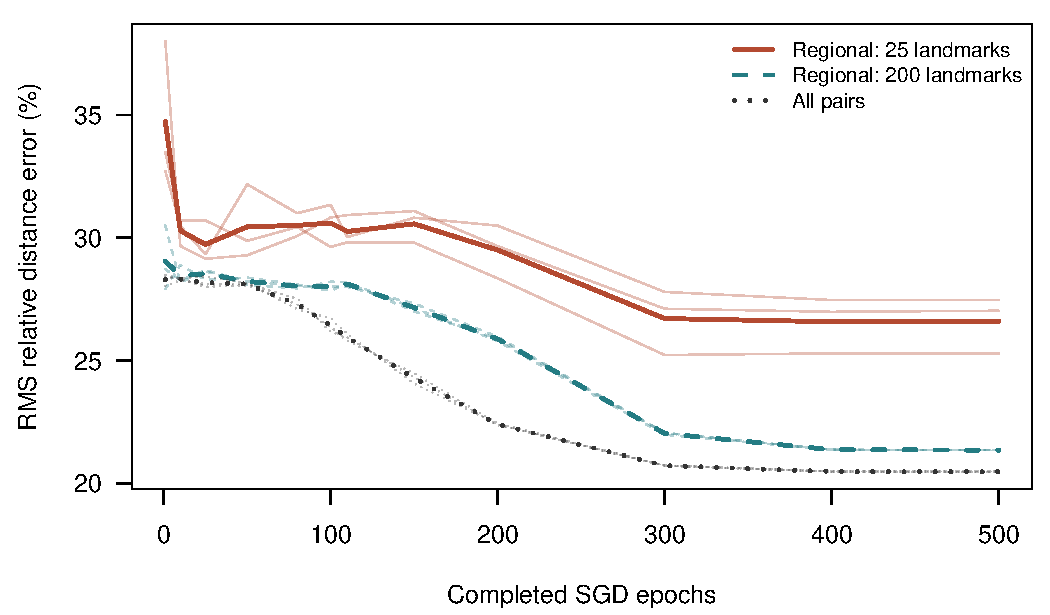
\includegraphics[width=\linewidth]{error-trajectories.pdf}
\caption{Exact all-pairs RMS relative error across the fixed 500-epoch
schedule. Thin curves show individual starts; thick curves show their
arithmetic means. Color and line style distinguish methods. The initial
configuration at epoch zero is omitted to make changes during fitting
readable. No confidence band is shown along the trajectories because three
starts provide limited information; final paired intervals are shown below.}
\end{figure}
\FloatBarrier

The trajectories answer two different questions. Early fluctuation occurs
even for the all-pairs reference, whose fitting terms exactly match the
evaluation objective. Thus objective mismatch is not necessary for
nonmonotonicity. Nevertheless, the regional methods and reference do not
end at the same error. Their final differences must be interpreted alongside
the sparse approximation, endpoint weighting, and method-specific rates,
not attributed to stochastic fluctuations alone.

\begin{table}[htbp]
\centering\begin{tabular}{lrrr}
\toprule
Method & Start 1 & Start 2 & Start 3 \\
\midrule
Regional: 25 landmarks & 25.290 & 27.030 & 27.469 \\
Regional: 200 landmarks & 21.352 & 21.352 & 21.354 \\
All pairs & 20.474 & 20.474 & 20.474 \\
\bottomrule
\end{tabular}

\caption{RMS relative distance error (percent) at epoch 500 for each
individual start. Starts 1--3 correspond to seeds 20190619--20190621.
Each column shares one starting configuration across methods.}
\end{table}

\begin{figure}[htbp]
\centering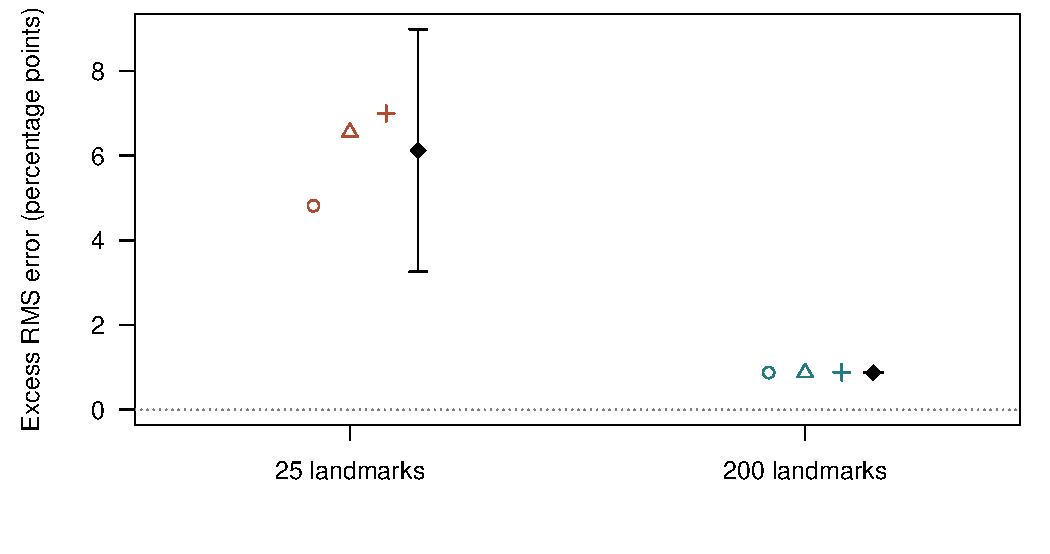
\includegraphics[width=\linewidth]{paired-differences.pdf}
\caption{Final paired differences: regional error minus the all-pairs error
from the same start, in percentage points. Positive values favor the
all-pairs reference. Three open symbols show the individual differences;
black diamonds and bars show the mean and a 95-percent paired $t$ interval
with two degrees of freedom. These intervals concern initialization
variability on this fixed subset and preparation, not generalization to
other cell samples or the full dataset.}
\end{figure}
\FloatBarrier

For three differences $\Delta_s=R_{{\rm regional},s}-R_{{\rm all},s}$,
$s=1,2,3$, the interval is
\begin{equation}
\bar\Delta\ \pm\ t_{0.975,2}\,
\frac{\sqrt{\sum_{s=1}^3(\Delta_s-\bar\Delta)^2/2}}{\sqrt3}.
\end{equation}
$\bar\Delta$ is the arithmetic mean and $t_{0.975,2}\simeq4.303$ is the
Student-$t$ quantile. With only three starts the approximate normality
assumption cannot be checked usefully. Individual values are therefore
shown, and the comparison is treated as a descriptive pilot.
At epoch 500, mean error is 26.596\% for 25 landmarks, 21.353\% for 200 landmarks, and 20.474\% for the all-pairs reference. Both regional methods have higher error than the reference in all three matched starts (zero better, zero tied, three worse for each comparison). For 25 landmarks the mean excess is 6.122 percentage points, with a paired 95-percent interval [3.259, 8.986]. For 200 landmarks it is 0.879 percentage points, with interval [0.875, 0.883]. The very narrow latter interval reflects similar final results across these three starts; it does not include cell-sampling or preparation uncertainty.

Increasing the landmark count reduces the observed approximation gap in this subset, but does not eliminate it. The experiment does not show that 200 landmarks are sufficient for another population, nor that the 2,000-landmark full fit will achieve these errors.


The proxy illustrates why the distinction matters: the 25-landmark method has a mean proxy RMS of 14.602\%, below 17.499\% for 200 landmarks, even though its all-pairs error is higher. Ranking these two fits by their own proxies would reverse the ranking given by the common evaluation metric. The all-pairs reference has equal proxy and evaluation values, 20.474\%, as required by the unit-multiplier identity.


\begin{figure}[htbp]
\centering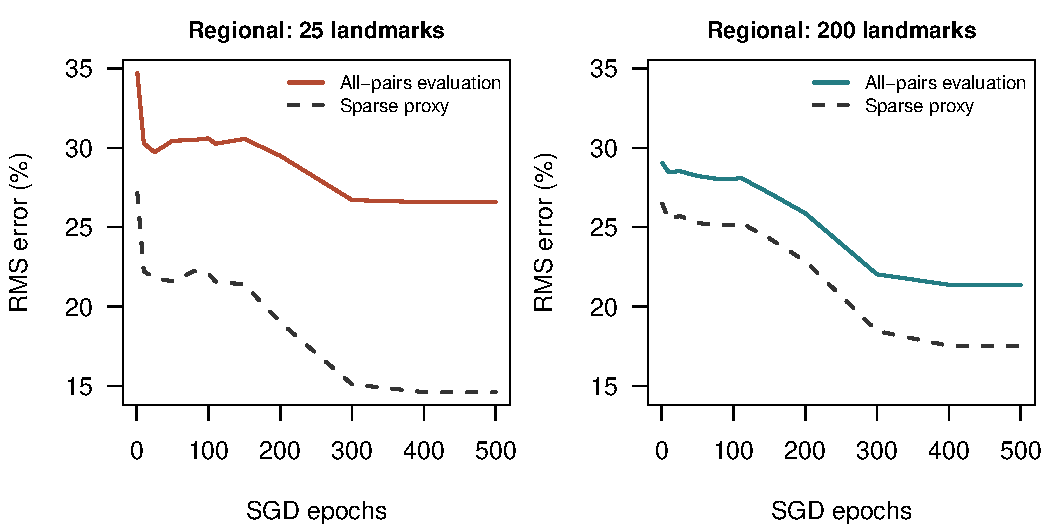
\includegraphics[width=\linewidth]{proxy-trajectories.pdf}
\caption{For each regional method, mean all-pairs evaluation and mean
endpoint-average proxy across the same three starts. Both are expressed
as RMS percentages, but have different pairs and weights. A gap is not
an optimization tolerance or a Monte Carlo error bar.}
\end{figure}
\FloatBarrier

\section{Checks and limits of interpretation}
The runner independently recomputes the proxy from coordinates and endpoint
counts at every checkpoint. For the all-pairs reference, that proxy equals
the independently computed full relative error to within $10^{-8}$
percentage points. The initial scalar scores match their common starting
configurations. A separate small test verifies that a four-epoch run followed
by six resumed epochs produces exactly the same coordinates as one
ten-epoch run with the same schedule.

Regional target distances are checked against the original PC20 Euclidean
distance matrix. A second script recomputes all 108 post-fit evaluations
row by row, independently of the runner's distance-vector calculation,
and checks agreement within $10^{-9}$ percentage points. Cache keys,
method identities, and seeds are also checked.
The nearest-neighbor diagnostic is
$n^{-1}\sum_i |N_i^{20}\cap N_i^{13}|/10$, where the sets contain the ten
nearest other cells in original and search coordinates, respectively.
It measures how much neighbor selection changes under projection; it
does not assess embedding quality. The projection affects the regional
local-pair set but not the all-pairs targets.
The mean retention of original 20-PC ten-neighbor sets under the 13-dimensional search projection is 69.83\%; the median is 70\% and the fifth percentile is 50\%. Thus high retained variance does not imply identical local interactions.


These tests establish consistency between the formulas, saved coordinates,
and reported numbers. They do not certify a global minimum, convergence,
or fidelity to an unknown biological manifold. Euclidean geometry in 20 PCs
is an explicit target here, not a claim about biological truth.
All evaluation pairs are also fitting pairs in the reference, so this is
an objective-recovery comparison, not prediction on held-out cells.

Only one cell subset and one preparation per landmark count were used.
More landmarks change both the represented interactions and the regional
partition. The schedules also change with the endpoint-weight range.
Therefore the result cannot isolate asymmetry, landmark number, or schedule
as the sole cause of a difference. A follow-up ablation would hold the pair
set fixed while comparing regional asymmetric counts, symmetric
endpoint-average counts, and unit counts, with clearly defined schedule
controls. Those fits are not included here.

\section{Output dimension with 1,814-PC targets}\label{sec:dimension}
The earlier comparison fixes the output dimension at three. A separate
experiment asks how much of the measured error can be reduced by allowing
more coordinates. This changes the input target as well as the question:
the same 1,500 cells are extracted from the previously verified
full-population 1,814-PC matrix. Those PCs retain 99.002235 percent of the
variance of the centered, unscaled, transformed 3,290-gene matrix across
120,804 cells. The projection is not refitted for the sparse-MDS input.
Consequently these scores must not be compared directly with the earlier
20-PC scores as if their denominators were unchanged.

Here $x_i\in\mathbb R^{1814}$, the targets remain
$d_{ij}=\|x_i-x_j\|_2$, and $y_i\in\mathbb R^d$, with
\[
d\in\{3,4,5,10,20,25,50,100,200,300\}.
\]
The all-pairs score $R$ and sparse proxy are still
Equations~\eqref{eq:full} and~\eqref{eq:proxy}; every evaluation uses all
1,124,250 pairs, in original distance units and without post-fit rescaling.
The 99-percent variance threshold describes the input projection, not a
guarantee of 1-percent relative-distance error.

\subsection{Matched settings and completed fits}
All dimensions share one preparation with 200 internally selected
distance-proportional landmarks, regional endpoint counts, and symmetric
union-of-10-nearest-neighbor local interactions. The preparation seed is
20261021. For neighbor selection only, a centered, unscaled PCA fitted to
the subset retains 506 dimensions and about 90.02 percent of the subset's
1,814-PC variance. Mean retention of the ten nearest neighbors relative
to search in all 1,814 PCs is 86.37 percent, using the same intersection
definition as above. Every target distance still uses all 1,814 PCs.
The preparation contains \dimensionfittedpairs\ positive-weight pairs.

Each dimension has one start, with seed 20190619 for initialization and
fitting. A common Gaussian matrix with 300 columns supplies the first $d$
columns, which are centered and scale-fitted by the earlier formula.
These are related, nested random starts, not identical configurations:
adding coordinates and refitting the starting scale changes distances.
The SGD backend uses the same weight-dependent schedule in every dimension,
with $T=100$ and $\epsilon=0.1$ in Equation~\eqref{eq:schedule}.
These are completed 100-epoch schedules, not the first 100 epochs of the
earlier 500-epoch schedule. There is no edge-KK refinement.

Ten fits were attempted and all ten completed 100 epochs; none failed,
were skipped, or were excluded. Ten single-threaded workers were launched,
with fewer remaining active as smaller jobs finished. Peak sampled
aggregate resident memory was 4.23 GiB, below the 50 GiB watchdog threshold.
Sampling every two seconds is a monitored stop condition, not an operating
system hard cap. Per-fit native workspace allowance was 4 GiB.
All final errors were independently recomputed through Gram-matrix
distances and agreed within $10^{-8}$ percentage points. These checks
verify the scores, not convergence or a globally optimal embedding.

\begin{figure}[htbp]
\centering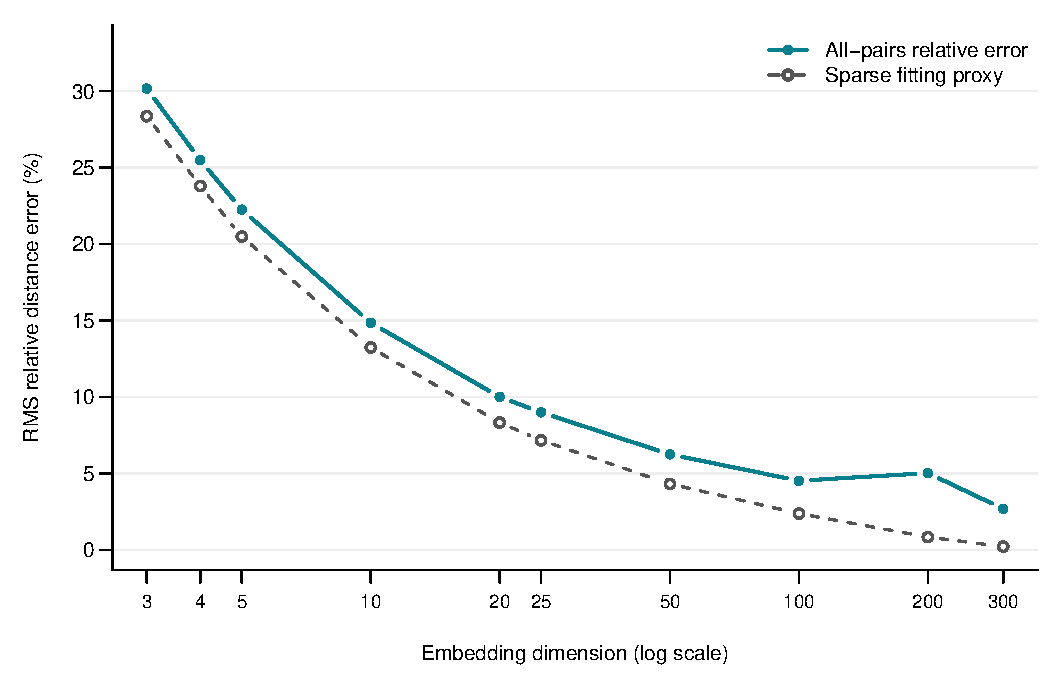
\includegraphics[width=\linewidth]{dimension-error.pdf}
\caption{Error after 100 SGD epochs versus output dimension for the same
1,500 cells and shared 200-landmark preparation. Filled teal points show
all-pairs RMS relative error; open gray points show the sparse proxy.
The horizontal axis is logarithmic; connecting segments guide the eye
between tested dimensions, not a fitted response curve. The all-pairs
error decreases substantially overall, but increases from 100D to 200D
even though the proxy continues to fall. No uncertainty band is available
from the single start per dimension.}
\label{fig:dimension}
\end{figure}

The all-pairs error falls from 30.164 percent in 3D to 10.000 percent in
20D and 2.680 percent in 300D. This is a substantial gain in reproducing
the chosen ambient distances, not evidence that biological geometry has
300 intrinsic dimensions. Dimensional restriction, the sparse approximation,
initialization and finite optimization all contribute to the achieved error.
In particular, the 200D score of 5.017 percent is higher than the 100D
score of 4.516 percent, despite a lower proxy (0.832 versus 2.371 percent).

\begin{table}[htbp]
\centering\begin{tabular}{rrr}\toprule
$d$ & All-pairs RMS (\%) & Sparse proxy RMS (\%) \\ \midrule
3 & 30.164 & 28.357 \\
4 & 25.483 & 23.791 \\
5 & 22.246 & 20.486 \\
10 & 14.850 & 13.230 \\
20 & 10.000 & 8.324 \\
25 & 8.987 & 7.158 \\
50 & 6.242 & 4.309 \\
100 & 4.516 & 2.371 \\
200 & 5.017 & 0.832 \\
300 & 2.680 & 0.210 \\
\bottomrule\end{tabular}

\caption{Terminal 100-epoch results on the 1,814-PC targets. $d$ is output
dimension; the all-pairs column is $R$ in Equation~\eqref{eq:full}, and
the proxy column is $100\sqrt{S_{\rm proxy}}$. Both are RMS percentages
but use different pair weights and denominators. Values are individual
fits, not means; one start per dimension does not support an uncertainty
interval. Lower values indicate closer distance agreement under the
respective score.}
\label{tab:dimension}
\end{table}
\FloatBarrier

\subsection{Where the 200D excess error occurs}
The proxy and the all-pairs score differ in two ways: which pairs contribute
directly, and how those pairs are weighted. To separate these effects,
let $F=\{\{i,j\}\in E:c_{ij}>0\}$ be the set of directly fitted pairs,
and let $U$ contain the remaining unordered pairs. Write $m_F=|F|$,
$m_U=|U|$, and $f=m_F/M$. Define the \emph{unweighted} RMS relative
error within each set by
\begin{equation}
R_A=100\sqrt{\frac{1}{|A|}\sum_{\{i,j\}\in A}
\left(\frac{r_{ij}-d_{ij}}{d_{ij}}\right)^2},\qquad A\in\{F,U\}.
\end{equation}
These scores give each pair equal weight within its own set. In contrast,
the proxy weights pairs in $F$ by $c_{ij}$. Since $F$ and $U$ partition
all pairs, their exact relationship to the overall score is
\begin{equation}\label{eq:partition}
R^2=fR_F^2+(1-f)R_U^2.
\end{equation}
Thus squared RMS percentages, not RMS percentages themselves, combine
linearly with the pair fractions.

There are $m_F=\dimensionfittedpairs$ directly fitted pairs
($\dimensionfittedfraction$ percent of all pairs) and
$m_U=\dimensionomittedpairs$ remaining pairs (74.18 percent).
The sets and weights are identical for the 100D and 200D fits.

\begin{table}[htbp]
\centering\begin{tabular}{rrrrr}\toprule
$d$ & $R$ & $R_F$ & $R_U$ & Proxy \\ \midrule
100 & 4.516 & 2.545 & 5.023 & 2.371 \\
200 & 5.017 & 0.896 & 5.801 & 0.832 \\
\bottomrule\end{tabular}

\caption{A diagnostic decomposition of the saved final fits, with no
rerunning of optimization. All numeric scores are RMS percentages.
$R$ evaluates all pairs equally; $R_F$ evaluates directly fitted pairs
equally; $R_U$ evaluates pairs absent from the fitting list equally.
``Proxy'' uses the regional endpoint-average weights on $F$.
The table isolates pair selection from reweighting within $F$.}
\label{tab:partition}
\end{table}
\FloatBarrier

The 200D fit improves agreement on the directly fitted pairs even without
their proxy weights: $R_F$ falls from 2.545 to 0.896 percent.
However, $R_U$ rises from 5.023 to 5.801 percent. Because $U$ contains
nearly three quarters of all pairs, its deterioration outweighs the
improvement on $F$ in Equation~\eqref{eq:partition}. This is the measured
reason for the higher overall RMS score. The discrepancy is not merely
a different normalization of two otherwise identical errors, nor only
reweighting within the fitting set.

Pairs in $U$ are not directly penalized by the sparse proxy, although their
distances can be influenced indirectly through shared cells, landmarks
and regional counts. They are not a statistically independent test set:
the same cells and input geometry helped construct the preparation and
the starting scale. The decomposition describes distance reconstruction,
not prediction on new cells.

Higher dimension itself cannot force a worse best attainable all-pairs
score. Appending 100 zero columns to a 100D configuration gives a feasible
200D configuration with exactly the same distances. Therefore
\begin{equation}
\inf_{Y\in\mathbb R^{1500\times200}}S_{\rm rel}(Y)
\ \leq\
\inf_{Y\in\mathbb R^{1500\times100}}S_{\rm rel}(Y).
\end{equation}
This statement concerns the best attainable score, not the terminal
configuration produced by a particular sparse-SGD run. The 200D run
reaches a configuration with better selected-pair agreement but worse
agreement elsewhere. Additional degrees of freedom, different starts,
and finite optimization can permit such outcomes; this experiment does
not isolate their separate contributions or establish that either fit
is trapped in a local minimum.

The 300D trace illustrates the same distinction over time: from epoch 10
to epoch 100 its proxy falls from 0.7724 to 0.2099 percent while its
all-pairs error rises slightly from 2.6183 to 2.6801 percent.
Useful diagnostics would repeat starts, increase landmark coverage, and
test a 200D warm start formed from the 100D result plus small nonzero extra
coordinates. Exactly zero extra coordinates alone would preserve the
lower-dimensional span under ordinary noncoincident pair updates.
Such diagnostics would be separate experiments, not replacements for
the results reported here.


\section{Consequences for grip and the full retinal experiment}
The distinction should be visible wherever sparse metric-MDS results are
reported: target geometry, update rule, sparse proxy, and independently
evaluated relative error are separate pieces of information.
For asymmetric regional fits, ``proxy'' is the appropriate label for the
endpoint-average scalar. For the all-pairs, unit-multiplier reference, the
same scalar really is the full relative-stress objective.

For fair comparisons of optimization trajectories, both methods should
report current, unrescaled coordinates at the same epoch. Best-checkpoint
selection and post-fit scale optimization may be useful output policies,
but must be identified and applied consistently if compared.
This experiment uses the current-state policy throughout.

The dimension sweep adds a concrete example of the distinction: a 200D
fit reproduces its selected interactions more closely than the 100D fit,
yet reproduces the remaining distances less accurately. Reporting only
the sparse proxy would reverse the ranking on the requested all-pairs score.

The small experiment tests the reason for fluctuations without restarting
the full job. It shows why stopping at epoch 100 need not reveal the outcome
of a 500-epoch schedule. It does not predict the final error of the paused
120,804-cell fit, nor show that increasing its landmark count is the right
next intervention. Its saved state at epoch 110 remains the valid restart
point; continuation should retain its original inputs, implementation
identity checks, random state, and schedule.

\section{Proposed comparison within developmental stages}
The pooled sample mixes developmental stages. Its dimension--error curve
therefore combines variation within stages with differences between them.
A natural next question is whether the curve is lower or has a different
shape within each stage. This section specifies a proposed experiment;
no stage-specific embeddings have yet been fitted.

There are ten annotated stages. Labels beginning with E denote embryonic
stages; labels beginning with P denote postnatal stages. Table~\ref{tab:stages}
shows the available cells. All stages contain at least 1,500 cells, so a
balanced comparison can draw a new uniform sample of 1,500 cells without
replacement \emph{within each stage}. Splitting the existing pooled
1,500-cell sample would instead give highly unequal, sometimes very small
groups (only 19 E12 cells), which is unsuitable for this comparison.

\begin{table}[htbp]
\centering\begin{tabular}{lrr}\toprule
Stage & Available cells & Proposed sample \\ \midrule
E11 & 9,364 & 1,500 \\
E12 & 1,610 & 1,500 \\
E14 & 26,944 & 1,500 \\
E16 & 5,401 & 1,500 \\
E18 & 23,011 & 1,500 \\
P0 & 9,925 & 1,500 \\
P2 & 17,963 & 1,500 \\
P5 & 6,756 & 1,500 \\
P8 & 11,727 & 1,500 \\
P14 & 8,103 & 1,500 \\
\bottomrule\end{tabular}

\caption{Available developmental-stage annotations in the 120,804-cell
input and the proposed sample size per stage. Counts are cells, not
biological replicates. Stages are ordered developmentally. No stage is
excluded under the proposed balanced sampling rule.}
\label{tab:stages}
\end{table}

For each sampled stage, keep the same full-population 1,814-PC coordinate
system and unscaled Euclidean target metric. Do not refit the input PCs,
whiten coordinates, or standardize each stage separately. The global
99.002235-percent variance retention does not imply that this exact fraction
holds within every stage. A stage-specific neighbor-search PCA retaining
90 percent of that stage sample's variance may still select local
interactions; as before, it must not change target distances.

Fit dimensions $d\in\{3,4,5,10,20,25,50\}$, with one shared preparation
per stage: 200 internally selected distance-proportional landmarks,
ten-neighbor local interactions, regional endpoint counts, and 100 SGD
epochs on a 100-epoch schedule with $\epsilon=0.1$. Use one explicitly
seeded start per stage and dimension for the first pass, with nested
starting-coordinate columns within a stage. Record sampling, preparation
and fitting seeds separately. This gives 70 planned fits, with no
resumption or modification of the paused full-population run.

Evaluate every within-stage unordered pair: 1,124,250 pairs per sample.
Report the all-pairs score and sparse proxy separately, retaining
ten-epoch histories and terminal coordinates without post-fit rescaling.
Show stage-specific curves on common axes, together with the existing
pooled-sample curve over the same dimensions. Retain directly fitted and
remaining-pair diagnostics when the scores disagree. A replenished queue
can use up to ten single-threaded workers under the same 50 GiB aggregate
resident-memory watchdog; preparation and fitting must share both this
memory allowance and the ten-thread CPU budget.

Interpret differences descriptively. The relative score divides each
residual by that stage sample's own target distance; target-distance
distributions can differ across stages. Lower error within a stage would
show easier reconstruction of that sample's Euclidean distances under
this method, not by itself lower biological intrinsic dimension or a
causal effect of age. Cell-type composition and sample or batch structure
may also differ. Equal cell counts control the number of pairs and the
landmark fraction, but do not remove these differences. Multiple starts
and independent cell subsamples should follow before making robust
comparisons between stages.
\FloatBarrier


\appendix
\section{Evidence and reproduction}
The exact input hash, cell indices, preparation objects, starting
coordinates, solver settings, and saved checkpoint coordinates are in the
private result bundle \path{retinal-relative-stress-20261020}.
Its protocol key begins \resultkey. Cell identifiers and raw expression
data are not distributed with this article. The compact
\texttt{scores.csv}, \texttt{fit-status.csv}, \texttt{preparations.csv},
and \texttt{paired-summary.csv} beside this source support the tables
and figures. The full source manifest and session information remain with
the private result bundle.

The experiment used the current optimized local grip and dgraphs builds.
The grip source baseline is commit \texttt{f3e570e1}; no solver code was
modified for this comparison. The paused large fit instead uses its
recorded frozen grip source, \texttt{348b16bb}. The intervening grip changes
add optional update tracing; tracing is disabled here. These are separate
experiments, not interchangeable checkpoints. Source fingerprints are
checked before and after the subset fits.

Implementation evidence is in \path{R/sparse_metric_mds.R} (weights,
normalization, proxy and terminal-coordinate policy),
\path{R/metric_mds_sgd.R} (schedule),
\path{src/sparse_metric_mds.cpp} (regional counts and local overrides),
\path{src/metric_mds_sgd.cpp} (pair updates and proxy),
and \path{R/metric_mds_continuation.R} (state integrity and resumption).
This note makes no literature-priority claim for these algorithms.

The reproducible scripts have separate roles.
\texttt{compare.R} generates fits; \texttt{validate.R} independently checks
their scores and neighbor retention; \texttt{summarize.R} creates tables and
figures; \texttt{build.R} refreshes the Eastern build timestamp and compiles
the PDF twice. The adjacent README gives arguments and commands.
The result-generation timestamp is \resultgenerated; the PDF build timestamp
is \reportbuilddatetime.

The recorded \texttt{fit.seconds} values measure accumulated elapsed time
inside the initial fitting call and subsequent continuation calls. They
include interface validation and saved-state integrity work, but exclude
separate data/preparation construction, external evaluation, output writing,
and figure rendering. They are not end-to-end runtime benchmarks.

The additional dimension experiment has a separate private result bundle:
\begin{quote}\small\path{retinal-dimension-sweep-pc1814-20261020}\end{quote}
Its \texttt{prepared.rds} stores the input and shared preparation;
dimension-specific fits store restartable states and ten-epoch score histories.
The coordinator \texttt{dimension-sweep.py} manages workers and memory;
\texttt{dimension-sweep.R} fits embeddings, and
\texttt{dimension-validate.R} independently checks final errors.
Fits completed at \dimensiongenerated, without solver changes.

The report-only script \texttt{dimension-report.R} generates the vector plot,
tables, pair-set decomposition, and stage counts. The scores are in
\texttt{dimension-summary.csv}; companion CSV files give the decomposition
and stage counts. These compact results accompany the source; cell identifiers,
large objects and logs remain private. The README gives reproduction commands.
Rendering neither reruns fits nor launches the proposed stage comparison.
\end{document}
